\section{Přechodné jevy prvního řádu}

\subsection{Sériový RC obvod}

Uvažujme elektrický obvod na obrázku \ref{fig:prvni_rad_rc} tvořený rezistorem $R$ a kapacitorem $C$. Kapacitor je nabit na počáteční  napětí $U_\mathrm{CO}$. Naším cílem je získat časový průběh napětí $u_\mathrm{C}(t)$ na capacitoru a proudu $i(t)$ obvodem.
\begin{figure}[h!]
\centering
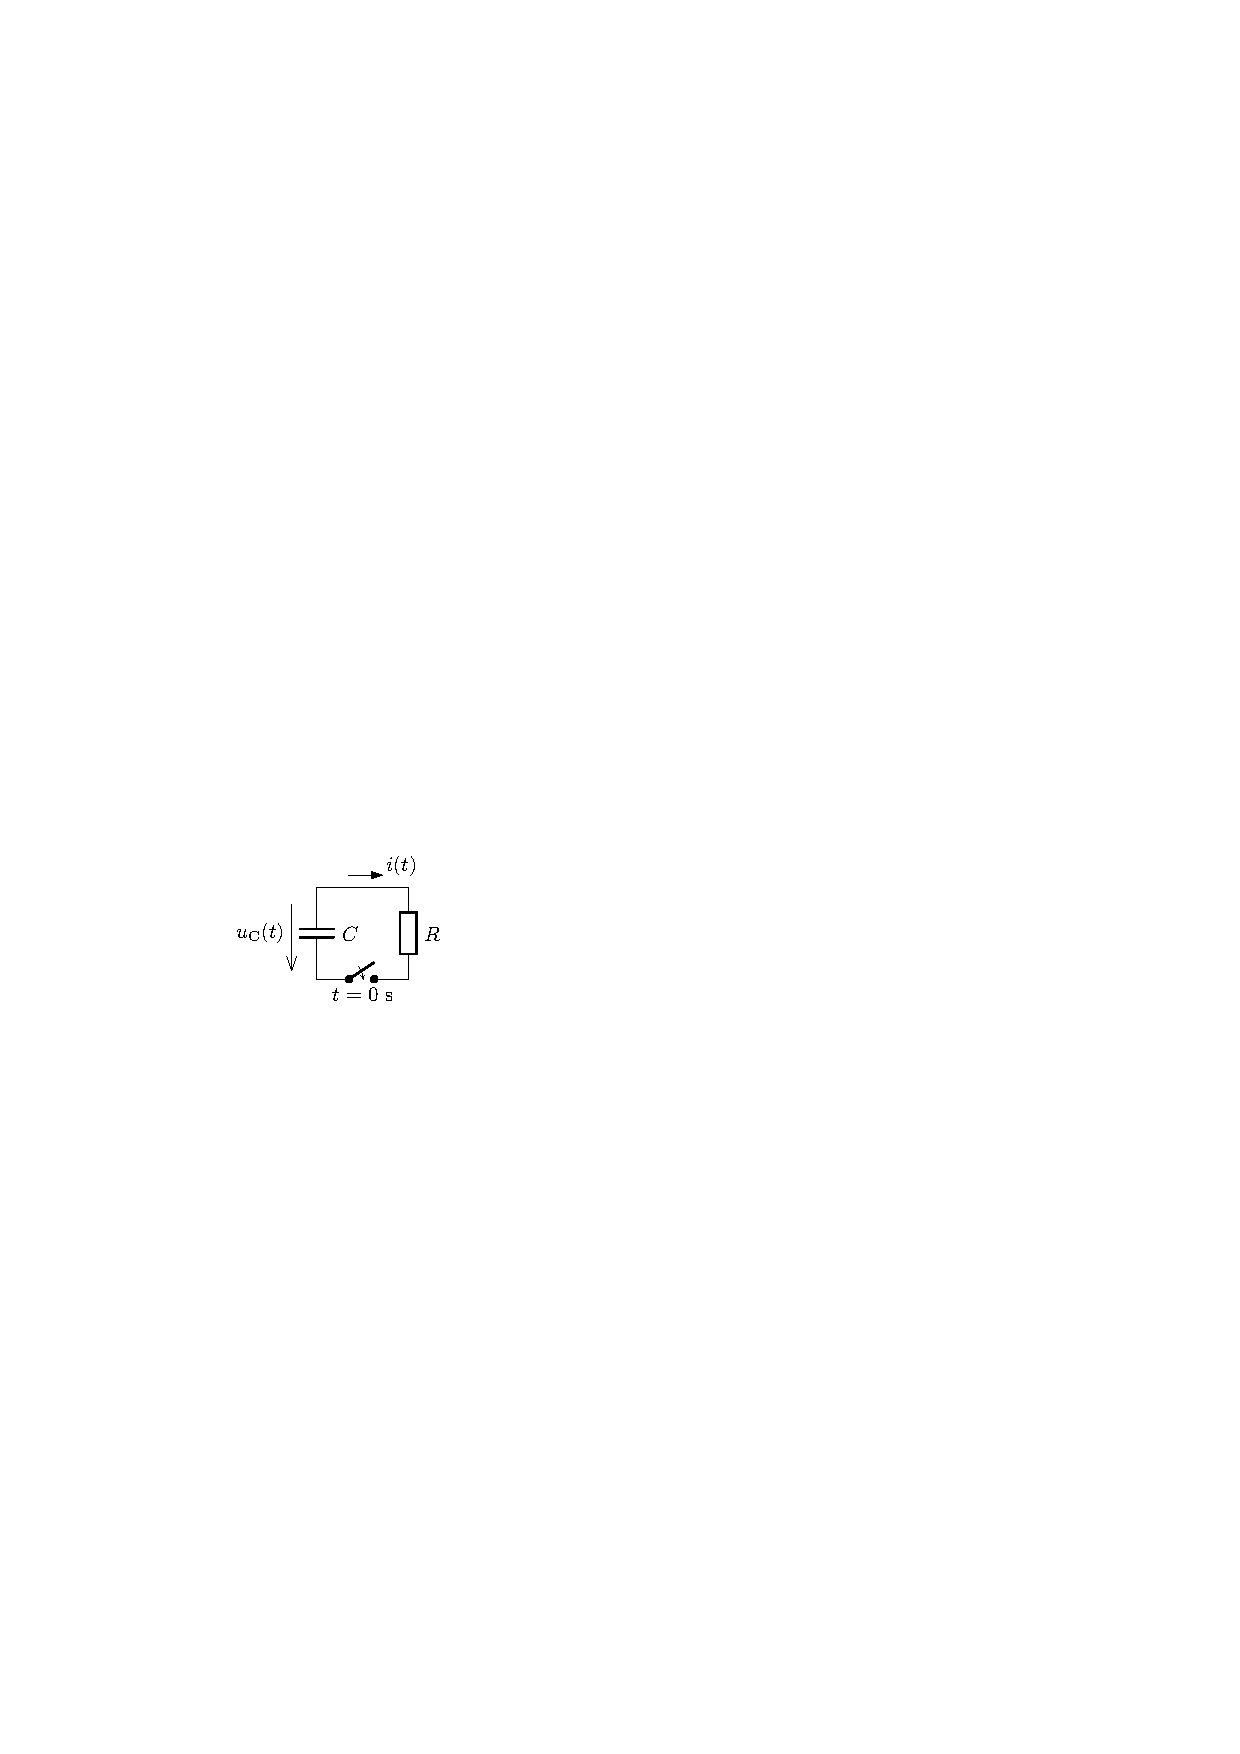
\includegraphics[]{prechodne_jevy/prvni_rad/rc.pdf}
\caption{Obvod prvního řádu s rezistorem a kapacitorem}
\label{fig:prvni_rad_rc}
\end{figure}
Kapacitor je nabit na napětí $U_\mathrm{CO}$, ze spojitosti stavové proměnné předpokládáme počáteční podmínku ve tvaru
$$
u_c(0-) = u_c(0+) = U_\mathrm{CO}.
$$
S využitím napěťového Kirchhoffova zákona lze zapsat napětí v uzavřené smyčce 
$$
Ri + u_\mathrm{C} = 0.
$$
Proud obvodem lze vyjádřit ve tvaru 
$$
i = C \frac{\dif u_\mathrm{C}}{\dif t}.
$$
Diferenciální rovnice popisující časový průběh proudu v obvodu je
\begin{equation}
RC \frac{\dif u_\mathrm{C}}{\dif t} + u_\mathrm{C} = 0.
\label{eq:prvni_rad_rc_dif_rce}
\end{equation}
Řešení diferenciální rovnice sestává z obecného $u_o$ a partikulárního řešení $u_p$
$$
u_\mathrm{C} = u_o + u_p.
$$
Řešení obecné diferenciální rovnice (rovnice s nulovou pravou stranou) předpokládáme ve tvaru
$$
u_o = K \cdot \me^{\lambda t},
$$
kde $K$ a $\lambda$ jsou neznámé konstanty. Konstantu $\lambda$ získáme řešením charakteristické rovnice\footnote{Charakteristickou rovnici získáme tak, že do diferenciální rovnice dosadíme předpokládaná řešení stavové proměnné.} k diferenciální rovnici (\ref{eq:prvni_rad_rc_dif_rce})
$$
RC \cdot \lambda + 1 = 0.
$$
Zápornou převrácenou hodnotu řešení charakteristické rovnice $\lambda = - \frac{1}{RC}$
$$
\tau = - \frac{1}{\lambda} = RC
$$ 
nazýváme časovou konstantou. 

Partikulární řešení představuje ustálený stav. Je zřejmé, že po odeznění přechodného děje bude kapacitor plně vybit
$$
u_p = u_\mathrm{C}(\infty) = 0.
$$
Napětí na kapacitoru získáme jako součet obecného a partikulárního řešení ve tvaru
$$
u_\mathrm{C} = u_o + u_p = K \cdot \me^{-\frac{t}{RC}}.
$$
Aplikujeme počáteční podmínku napětí na kapacitoru $u_c(0+) = U_\mathrm{CO}$
$$
U_\mathrm{CO} = K \cdot \lim_{t \rightarrow 0} \left( \me^{-\frac{t}{RC}} \right) = K
$$
a ihned získáme neznámou konstantu $K = U_\mathrm{CO}$. Časový průběh napětí na kapacitoru $u_c(t)$ je zobrazen na obrázku \ref{fig:prvni_rad_rc_graf_u} a lze vyjádřit ve tvaru
\begin{equation}
u_\mathrm{C} = U_\mathrm{CO} \cdot \me^{-\frac{t}{RC}}.
\label{eq:prvni_rad_rc_u}
\end{equation}
\begin{figure}[h!]
\centering
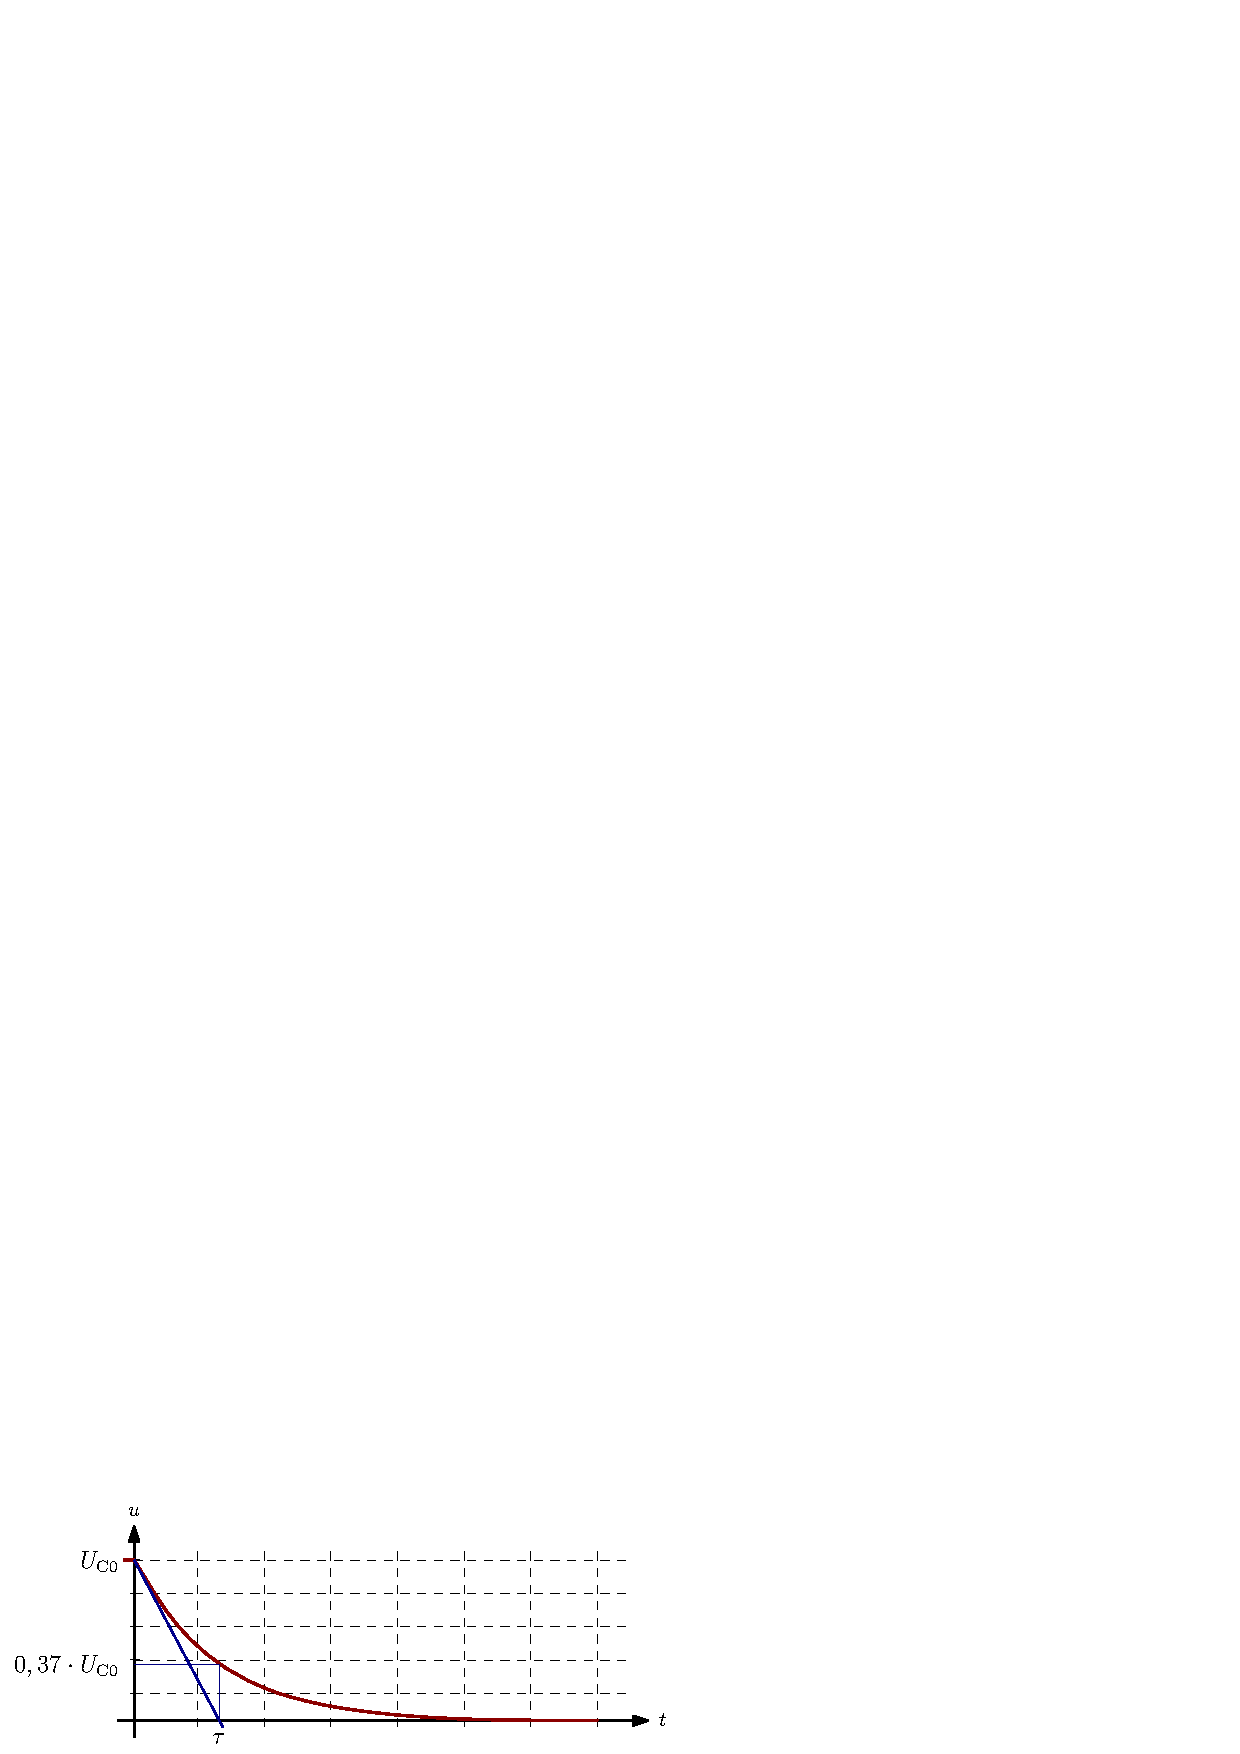
\includegraphics[]{prechodne_jevy/prvni_rad/rc_graf_u.pdf}
\caption{Časový průběh napětí na kapacitoru}
\label{fig:prvni_rad_rc_graf_u}
\end{figure}
Proud obvodem vidíme na obrázku \ref{fig:prvni_rad_rc_graf_i} a získáme ho derivací napětí na kapacitoru
$$
i = C \frac{\dif u_\mathrm{C}}{\dif t} = - \frac{U_\mathrm{CO}}{R} \cdot \me^{-\frac{t}{RC}}.
$$
\begin{figure}[h!]
\centering
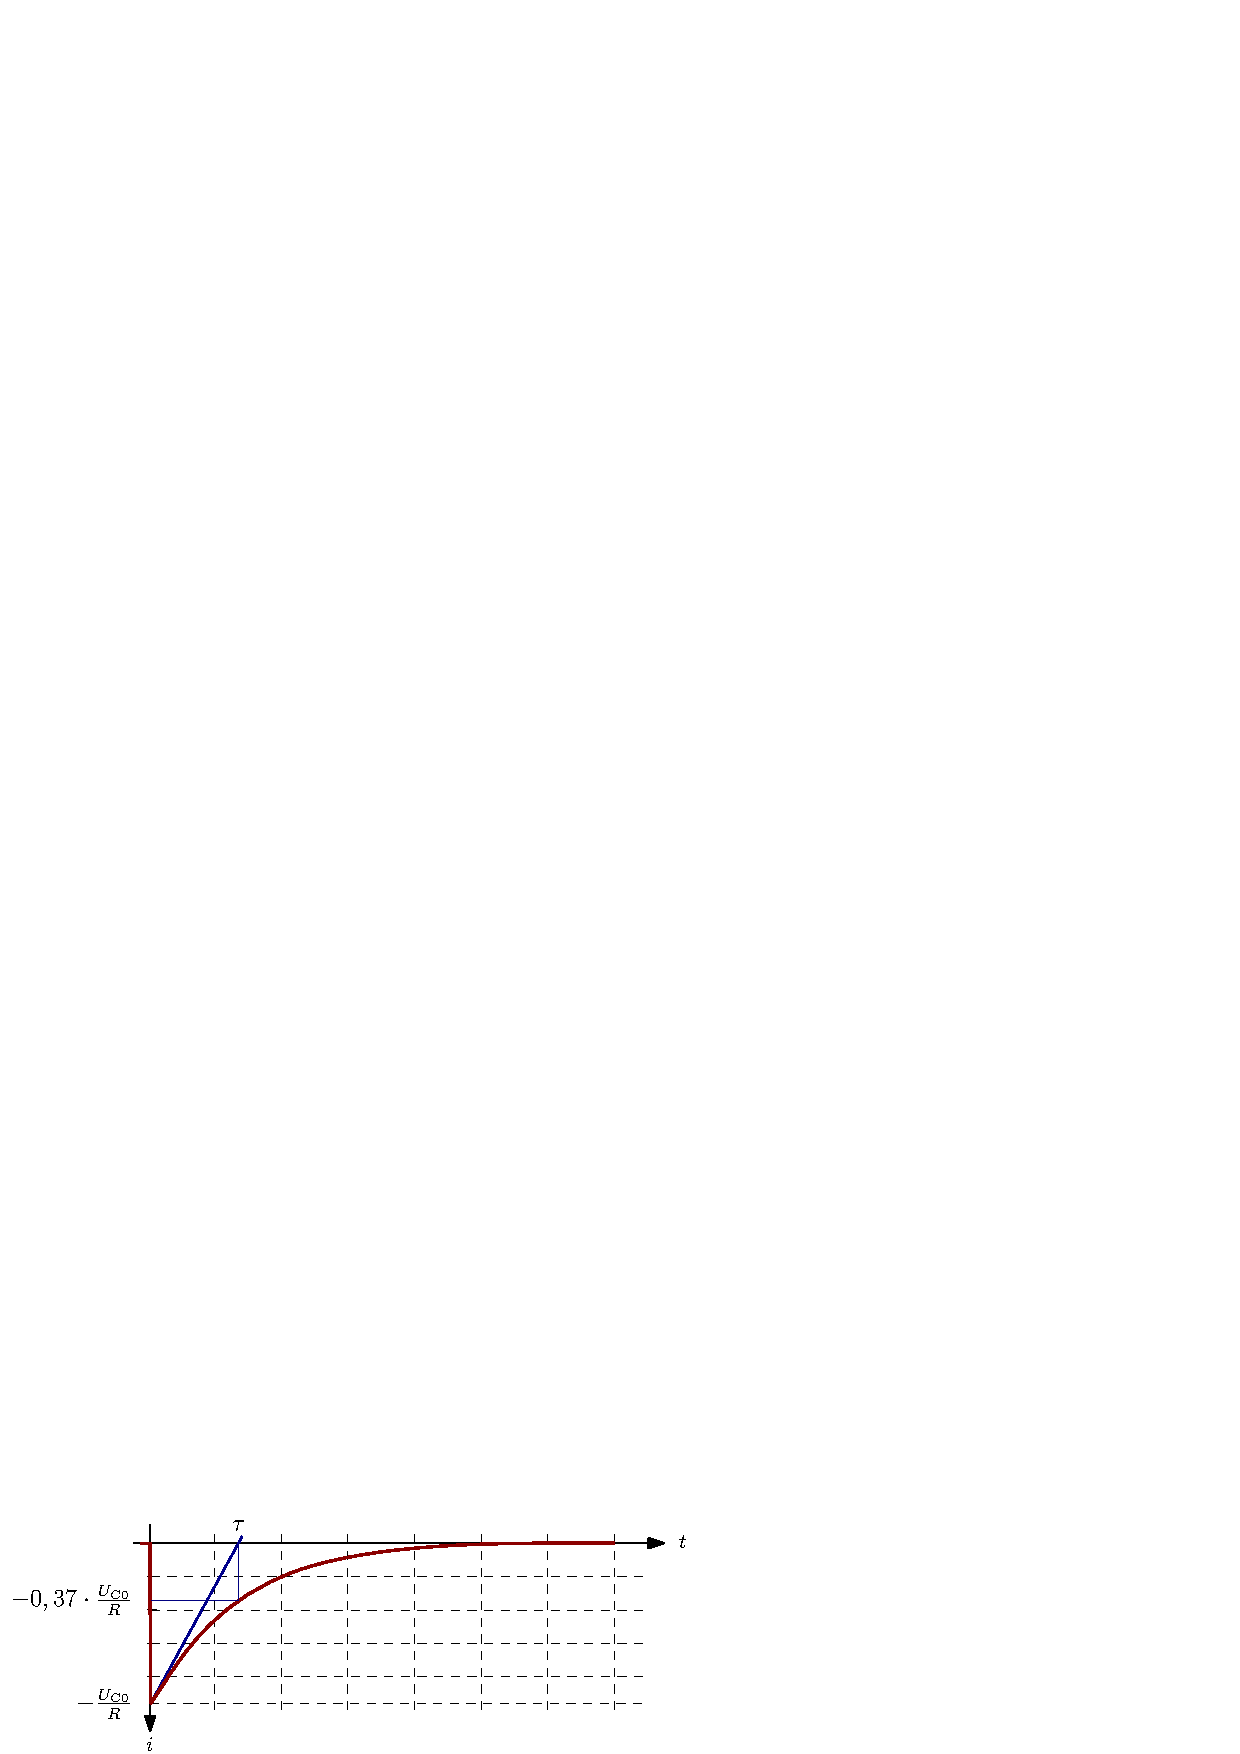
\includegraphics[]{prechodne_jevy/prvni_rad/rc_graf_i.pdf}
\caption{Časový průběh proudu v obvodu}
\label{fig:prvni_rad_rc_graf_i}
\end{figure}

Význam časové konstanty je patrný z následující úvahy. Nejprve dosadíme za čas do vztahu (\ref{eq:prvni_rad_rc_u}) časovou konstantu $\tau$ a získáme
$$
u_\mathrm{C}(\tau) = U_\mathrm{CO} \cdot \me^{-\frac{\tau}{\tau}} = U_\mathrm{CO} \cdot \me^{-1} = 0,368 \cdot U_\mathrm{CO}.
$$
Je zřejmé, že za dobu jedné časové konstanty klesne napětí na kapacitoru na 37 \% napětí na počátku přechodného děje. Z obrázku \ref{fig:prvni_rad_rc_graf_tau} je patrný vliv velikosti časové konstant na rychlost přechodného děje. Menší hodnota časové konstanty způsobí rychlejší dosažení ustáleného stavu. Obvod můžeme považovat za ustálený za dobu $5\tau$ kdy napětí klesne na 0,7~\% své původní hodnoty.
\begin{figure}[h!]
\centering
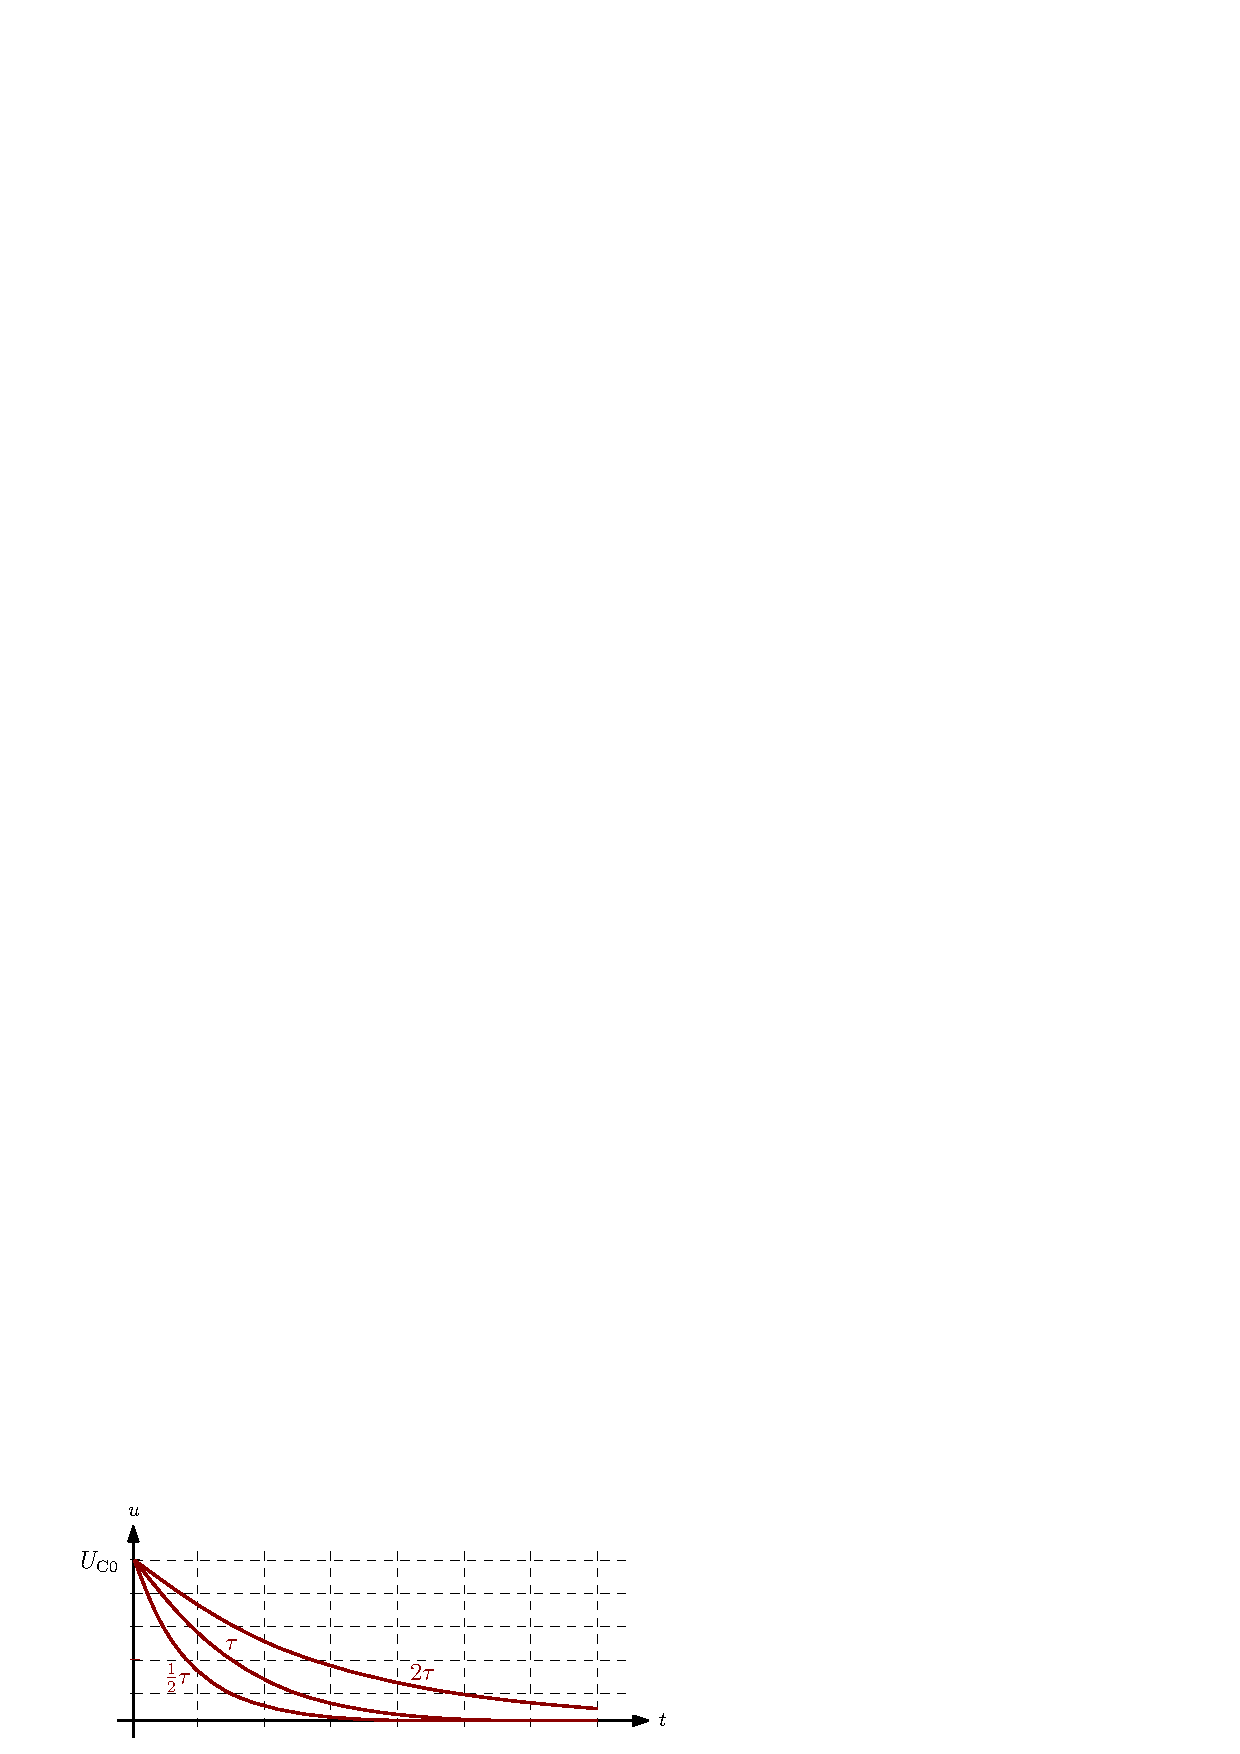
\includegraphics[]{prechodne_jevy/prvni_rad/rc_graf_tau.pdf}
\caption{Vliv časové konstanty na rychlost přechodného děje}
\label{fig:prvni_rad_rc_graf_tau}
\end{figure}

\subsubsection{Sériový RL obvod}

Uvažujme elektrický obvod na obrázku \ref{fig:prvni_rad_rl} tvořený rezistorem $R$ a induktorem $L$ napájený zdrojem napětí $U_0$. 
\begin{figure}[h!]
\centering
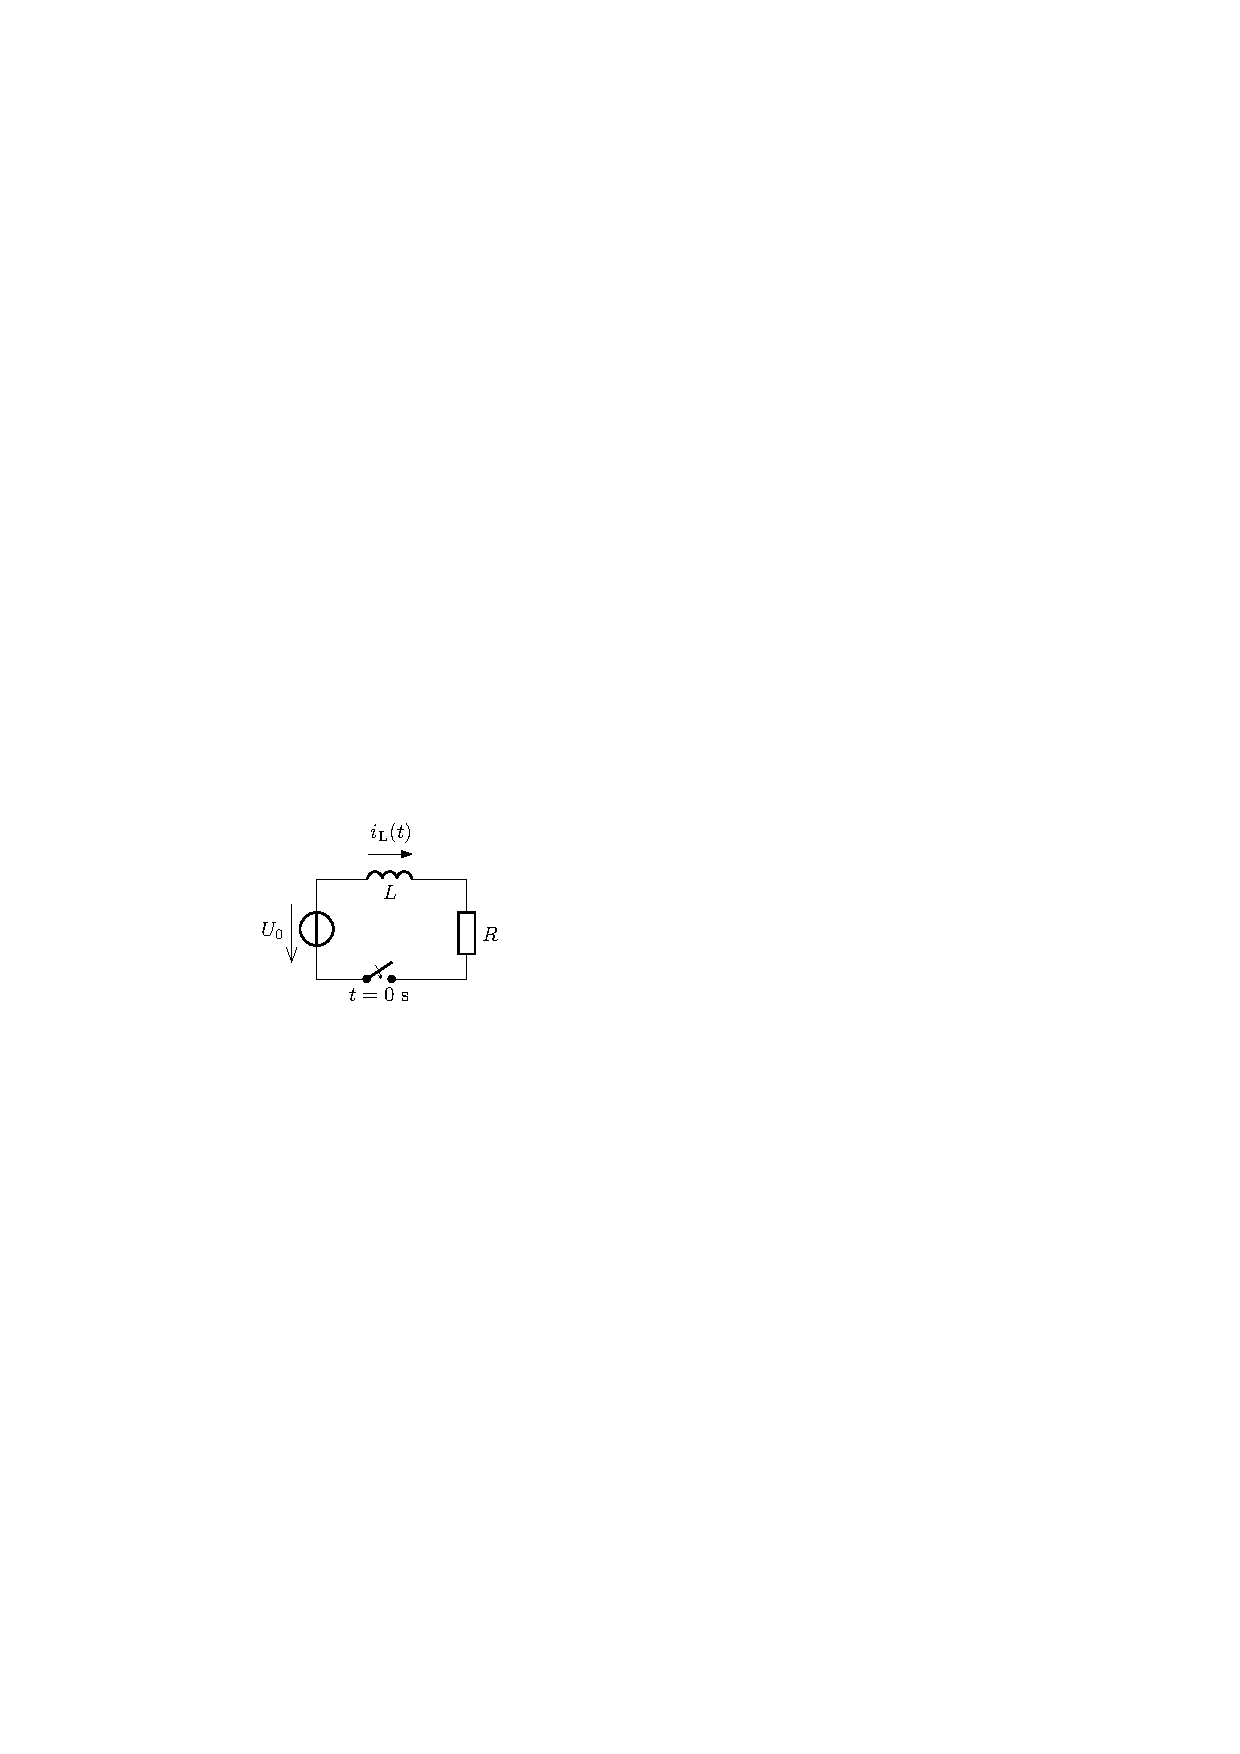
\includegraphics[]{prechodne_jevy/prvni_rad/rl.pdf}
\caption{Obvod prvního řádu s rezistorem a induktorem}
\label{fig:prvni_rad_rl}
\end{figure}

\begin{figure}[h!]
\centering
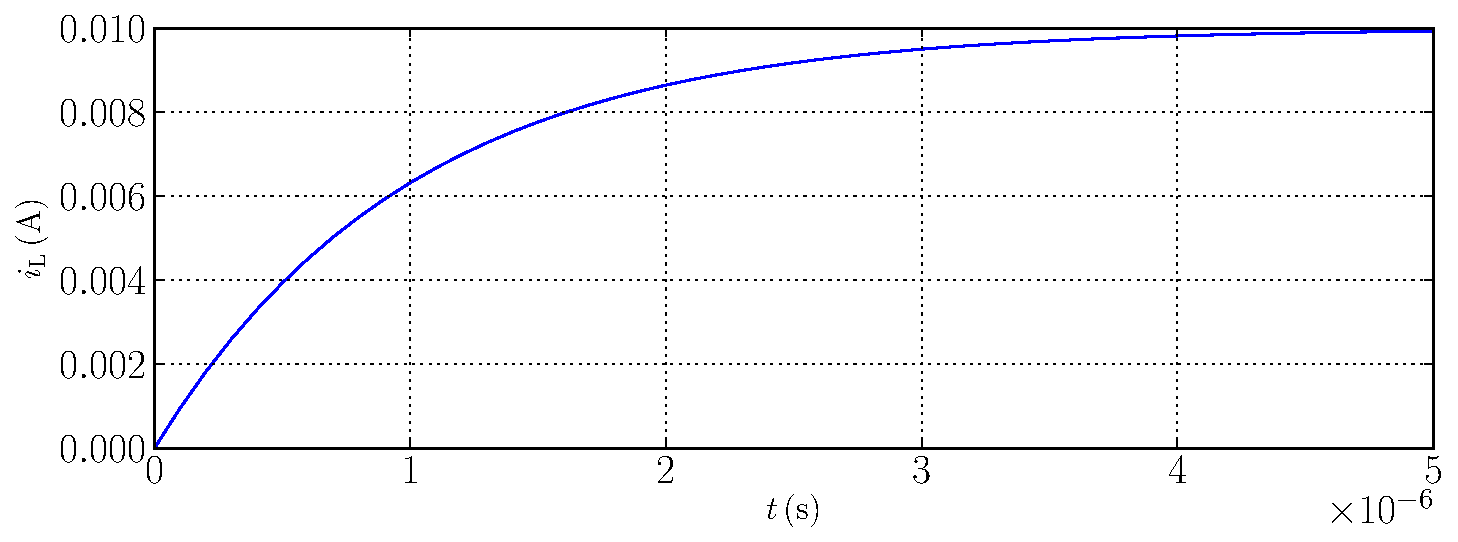
\includegraphics[width=13cm]{prechodne_jevy/prvni_rad/obvod_rl_proud.pdf}
\caption{Sériový RL obvod: proud induktorem}
\label{fig:obvod_rl_proud}
\end{figure}
